% !TeX document-id = {87432cc9-c386-48dc-9558-b3c42a74a150}
% !TEX encoding = UTF-8
% !TEX TS-program = pdflatex
% !TEX spellcheck = it-IT
%% !TEX root = 
% !BIB TS-program = biber
% Comandi speciali (o righe magiche) trattati come commenti da Latex ma non da 
%editor come Texstudio e Texshop, che si impostano di conseguenza. In ordine:
% dichiara la codifica dei caratteri con cui impostare l'editor (bisogna 
%comunque caricare inputenc con la stessa codifica)
% dichiara il motore di composizione (pdflatex o lualatex)
% attiva il controllo ortografico della lingua del documento
% dichiara la condizione di file principale e di file secondario nei documenti 
%suddivisi in più file
% imposta biber come motore bibliografico

\documentclass[9pt]{extarticle}


% ------------------------------------------------------------------------------
% Packages
% ------------------------------------------------------------------------------
\usepackage[utf8]{inputenc}
\usepackage{graphicx}
\usepackage{amsmath}
\usepackage{amssymb}
\usepackage{amsthm}
\usepackage{hyperref}
\usepackage{titlesec}
\usepackage{parskip}
\usepackage{float}
\usepackage{booktabs}
\usepackage{caption}
\usepackage{blindtext}
\usepackage[table,xcdraw]{xcolor}
\usepackage{enumitem}
% Define a new counter for functional requirements
\newcounter{rf}
\newcommand{\FR}{\refstepcounter{rf}\textbf{FR\therf: }}
% Define a new counter for non-functional requirements
\newcounter{nonfunc}
\newcommand{\NONFUNC}{\refstepcounter{nonfunc}\textbf{NFR\thenonfunc: }}

% ------------------------------------------------------------------------------
% Page setup
% ------------------------------------------------------------------------------
\usepackage{geometry} 
\geometry{a4paper, margin=1in, twoside}
\usepackage{setspace}
\setstretch{1.2}  % Adjust the number as needed
%\doublespacing


% ------------------------------------------------------------------------------
% Referencing
% ------------------------------------------------------------------------------
\usepackage[
	backend=biber,
	citestyle=authoryear,
	bibstyle=authoryear,
	maxcitenames=2,
	maxbibnames=99]{biblatex}
%\addbibresource{references.bib}
%\DeclareNameAlias{sortname}{family-given}
%\setlength\bibitemsep{1em}

% ------------------------------------------------------------------------------
% Code listings
% ------------------------------------------------------------------------------
\usepackage{listings}
\usepackage{xcolor}
\lstdefinestyle{matlabcode}{
	backgroundcolor=\color{gray!10},   
	commentstyle=\color{green!50!black},
	keywordstyle=\color{blue},
	stringstyle=\color{magenta},
	basicstyle=\linespread{1}\footnotesize\ttfamily,
	numberstyle=\tiny,
	breakatwhitespace=false,         
	breaklines=true,                 
	captionpos=t,   
	frame=single,
	keepspaces=true,         
	language=matlab,        
	numbers=none,             
	numbersep=5pt,                  
	showspaces=false,                
	showstringspaces=false,
	showtabs=false,                  
	tabsize=2,
	aboveskip=1em,
	belowskip=1em,
	belowcaptionskip=12pt
}

% ------------------------------------------------------------------------------
% Headers and footers
% ------------------------------------------------------------------------------	
\usepackage{fancyhdr}
\pagestyle{fancy}   
\setlength{\headheight}{14.5pt}
\renewcommand{\headrulewidth}{0.3pt}
%\renewcommand{\chaptermark}[1]{\markboth{\chaptername\ \thechapter.\ #1}{}}
\renewcommand{\sectionmark}[1]{\markright{\thesection.\ #1}}   
\fancyhead[LE,RO]{\rightmark}
\fancyhead[LO,RE]{\leftmark}

% ------------------------------------------------------------------------------
% Title page
% ------------------------------------------------------------------------------

\newcommand{\name}{Togni Roberto}
\newcommand{\projecttitle}{EvenTrento}
\newcommand{\course}{Ingegneria del Software}
\newcommand{\customtitle}{
	\vspace*{1cm}
	\begin{center}
		
\includegraphics[width = 7cm]{images/logo_rosso} \\
		\vspace{1cm}
	\end{center}
	\LARGE{Progetto:}
	\begin{center}
%		\vspace{2cm}
		\textbf{\Huge{\projecttitle}} \\
	\end{center}
	\LARGE{Titolo del documento:}
	\begin{center}
%		\vspace{1cm}
		\textbf{\Huge Descrizione di Progetto} \\
	\end{center}
	\LARGE{Autore:}
	\begin{center}
		%		\vspace{1cm}
		\textbf{\name} \\
	\end{center}
	\vspace{1cm}
	Document Info:
	
	\begingroup
	\setlength{\tabcolsep}{10pt} % Default value: 6pt
	\renewcommand{\arraystretch}{1.5}
	
	\begin{table}[!htb]
		\begin{tabular}{lllll}
			\cline{1-4}
			\cellcolor[HTML]{13315C}{\color[HTML]{FFFFFF} Doc. Name}                         & D1-EvenTrentoDescrizioneProgetto & \multicolumn{1}{l|}{\cellcolor[HTML]{13315C}{\color[HTML]{FFFFFF} Doc. Number}} & \multicolumn{1}{l|}{D1 V0.1} &  \\ \cline{1-4}
			\multicolumn{1}{|l|}{\cellcolor[HTML]{13315C}{\color[HTML]{FFFFFF} Description}} & \multicolumn{3}{l|}{Documento di analisi dei requisiti funzionali, non funzionali e front-end}                                                    &  \\ \cline{1-4}
			&                                  &                                                                                 &                              &  \\
			&                                  &                                                                                 &                              &  \\
		\end{tabular}
	\end{table}
	
	\endgroup
	
	\begin{center}
		\vfill 
		\textbf{\Large Dipartimento di Ingegneria e Scienza dell'Informazione}
		\vspace{1cm}
	\end{center}
	\newpage
	\pagenumbering{roman}
	\setcounter{page}{0}
}

% ------------------------------------------------------------------------------
% Theorem enivornments
% ------------------------------------------------------------------------------
%\newtheorem{theorem}{Theorem}[chapter]
%\newtheorem{definition}{Definition}[chapter]
%\newtheorem{corollary}{Corollary}[theorem]
%\newtheorem{lemma}[theorem]{Lemma}

\newtheoremstyle{break}%
    {}{}%
    {}{}%
    {\bfseries}{}% % Note that final punctuation is omitted.
    {\newline}{}
\theoremstyle{break}
%\newtheorem{example}{Example}[chapter]



% ------------------------------------------------------------------------------
% Document
% ------------------------------------------------------------------------------


\begin{document}
\customtitle



% TODO add chapters
\tableofcontents
\newpage

\section{Scopo del documento}


Il seguente documento riporta la specifica dei requisiti funzionali del sistema tramite un linguaggio semi-formale. Si tratta dunque di un approfondimento (nonché di una formalizzazione) di quanto riportato in linguaggio naturale all'interno del D1. Il linguaggio utilizzato per la formalizzazione dei requisiti è UML (Unified Modeling Language), declinato in Use Case Diagrams (UCDs), Component Diagrams, Sequence Diagrams, e Class Diagrams.

\newpage

\section{Requisiti Funzionali}

Di seguito sono riportati i functional requirements (FR) del sistema sia in linguaggio naturale che tramite Use Case Diagrams (UCDs). La notazione è coerente con quella utilizzata all'interno del documento D1.



\subsection{FR1 e FR2: Login e Registrazione} 

\begin{figure}[!htb]
	\centering
	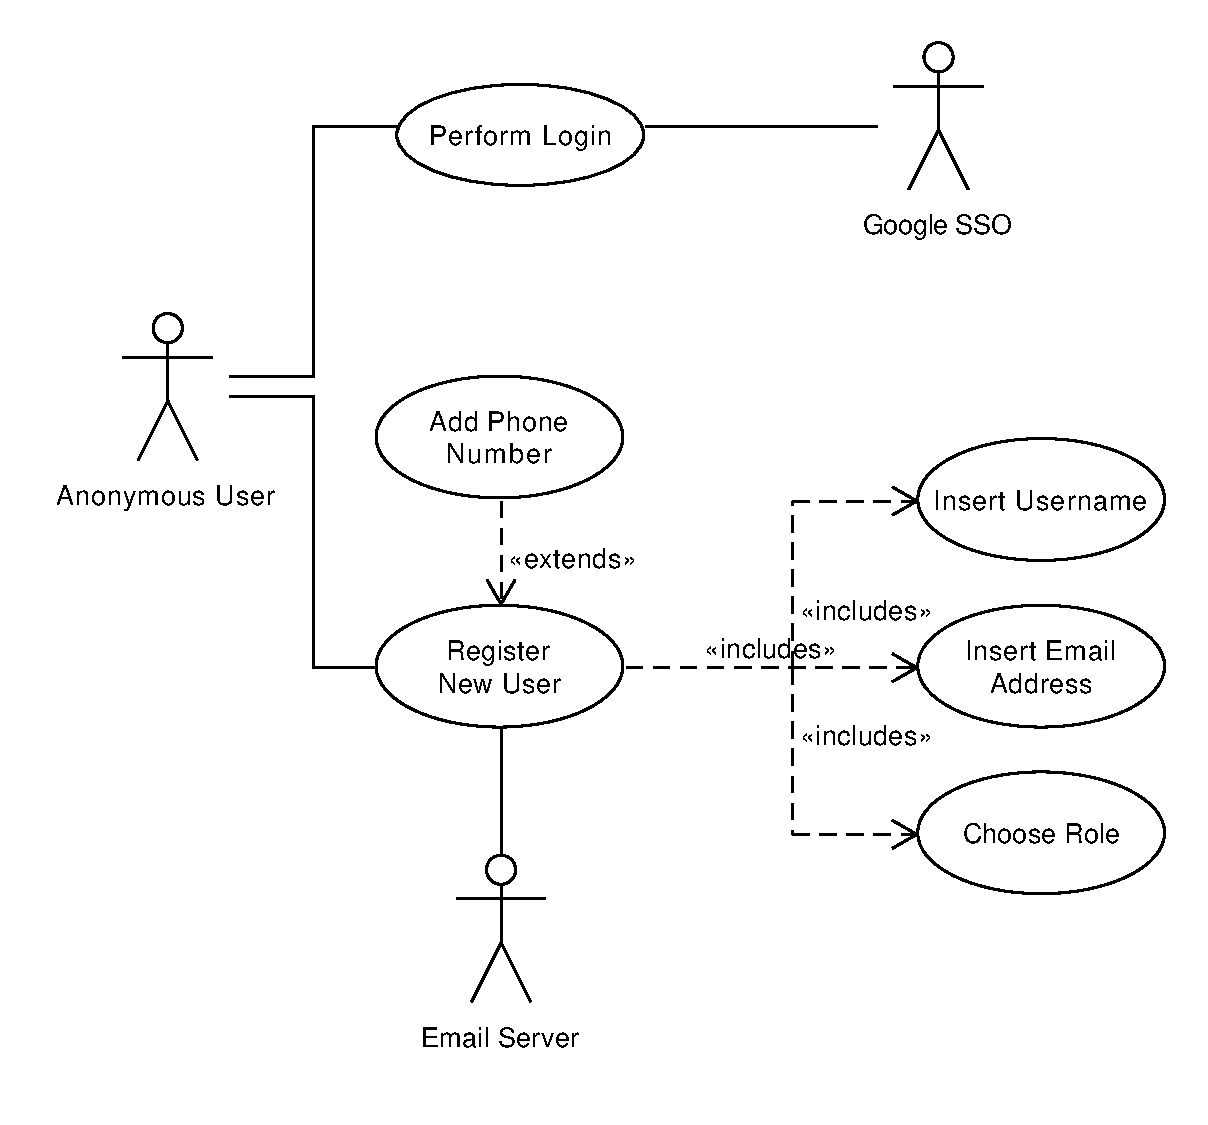
\includegraphics[width=.7\linewidth]{./images/FR1-2.pdf}
	\caption{UCD relativo a FR1 e FR2.}
	\label{fig:UCD_FR1-2}
\end{figure}

\subsubsection*{Use Case FR1: Login}

\textbf{Riassunto}

Lo use case in questione descrive come un utente può effettuare il login al sistema.

\textbf{Descrizione}

\begin{itemize}
	\item L'utente visualizza una pagina con un form
	\item Se l'utente inserisce le credenziali (vedi  \hyperref[Estensioni-FR2]{Estensioni}) corrette (vedi \hyperref[Eccezioni-FR2]{Eccezioni}) e preme sul pulsante "Login", si apre la schermata principale dell'applicazione.
	\item Qualora l'utente selezioni il logo di Google, il processo di autenticazione verrà gestito da Google SSO
\end{itemize}

\subsubsection*{Use Case FR2: Registrazione}

\textbf{Riassunto}

Lo use case in questione descrive come un utente può registrarsi al sistema.

\textbf{Descrizione}

\begin{itemize}
	\item L'utente visualizza una pagina dalla quale inserire nome, cognome, indirizzo mail (vedi \hyperref[Eccezioni-FR2]{Eccezioni})
	\item Il sistema invia una mail all'indirizzo fornito dall'utente contenente un link e una password temporanea
	\item L'utente deve confermare la registrazione tramite il link di cui sopra (vedi \hyperref[Eccezioni-FR2]{Eccezioni}). Può quindi accedere al sistema tramite la password temporanea
\end{itemize}


\subsubsection*{Eccezioni}\label{Eccezioni-FR2}

\begin{itemize}
	\item Qualora le credenziali inserite non siano corrette, l'applicazione restituisce un messaggio di errore
	\item Qualora l'utente non apra il link contenuto nella mail automatica, la registrazione non viene finalizzata
\end{itemize}

\subsubsection*{Estensioni}\label{Estensioni-FR2}

\begin{itemize}
	\item La password contenuta nella mail generata automaticamente dal sistema a seguito della registrazione dev'essere modificata a seguito del primo login
\end{itemize}

\subsection{FR4: Visualizzazione Eventi}

\begin{figure}[!htb]
	\centering
	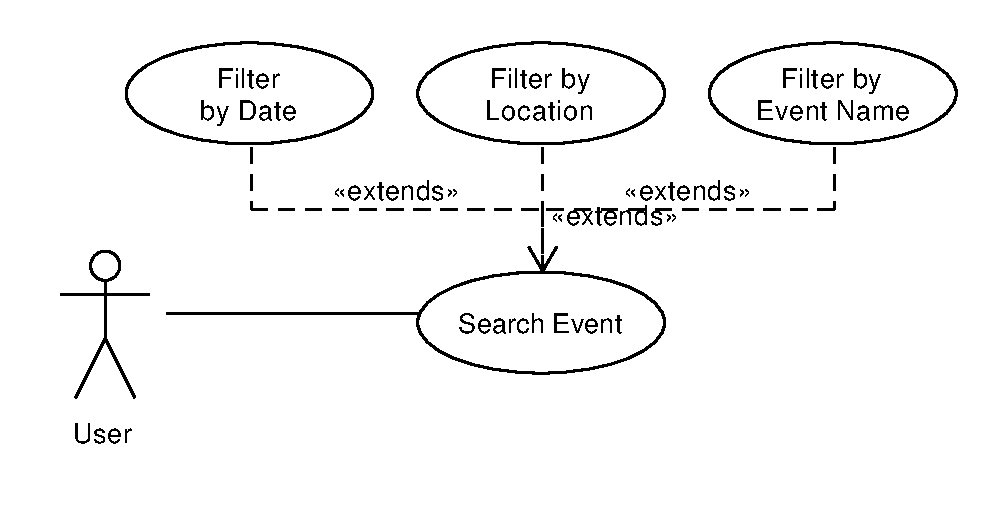
\includegraphics[width=.7\linewidth]{./images/FR4.pdf}
	\caption{UCD relativo al FR4.}
	\label{fig:UCD_FR4}
\end{figure}

\subsubsection*{Use Case FR4: Visualizzazione Eventi}

\textbf{Riassunto}

Lo use case in questione descrive come un utente può filtrare gli eventi presenti all'interno del sistema.

\textbf{Descrizione}

\begin{itemize}
	\item La ricerca di eventi può essere effettuata da qualsiasi utente, anche non loggato
	\item L'utente può scegliere se esplorare la mappa integrata nella schermata iniziale, o se visualizzare gli eventi in forma di lista
	\item Qualora l'utente decida di visualizzare la lista degli eventi, viene messo a disposizione un servizio di filtering basato su 3 possibili criteri: data, luogo e nome dell'evento
\end{itemize}

\subsection{FR5, FR6, FR16 e FR17: Feedback, Condivisione, Iscrizione e salvataggio Eventi}


\begin{figure}[!htb]
	\centering
	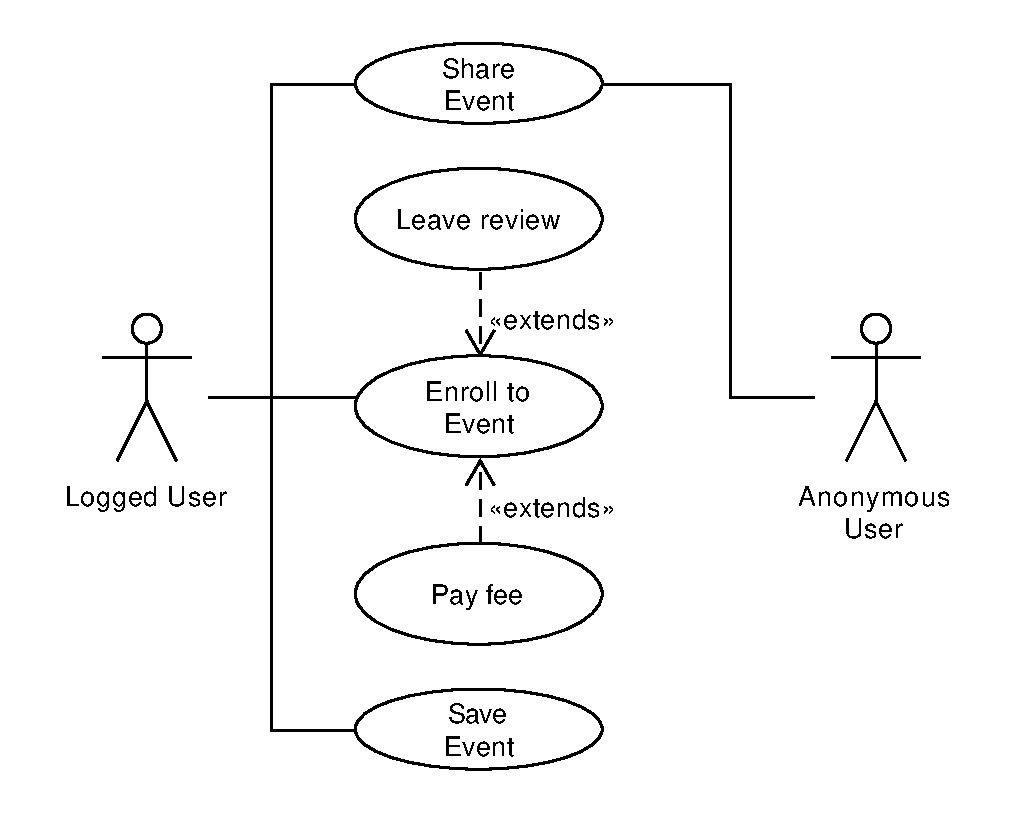
\includegraphics[width=.6\linewidth]{./images/FR5-6-16-17.pdf}
	\caption{UCD relativo a FR5, FR6, FR16 e FR17.}
	\label{fig:UCD_FR5-6-16-17}
\end{figure}

\subsubsection*{Use Cases FR5, FR6, FR16, FR17}

\textbf{Riassunto}

Lo use case in questione descrive come un utente può interagire con gli eventi offerti dal sistema. In particolare, descrive le attività di salvataggio, di iscrizione, di condivisione, nonché di valutazione della qualità di un evento.

\textbf{Descrizione}

\begin{itemize}
	\item Oltre a poter visualizzare gli eventi (come mostrato nello UCD precedente), qualsiasi utente può condividerli
	\item Previo login, qualsiasi tipologia di utente può salvare e/o iscriversi ad un evento. L'iscrizione comporta l'eventuale pagamento del biglietto
	\item Qualsiasi utente iscritto ad un evento può, dopo il suo verificarsi, lasciare una review
\end{itemize}


\subsection{FR8 e FR10: Creazione ed Aggiornamento Eventi}

\begin{figure}[!htb]
	\centering
	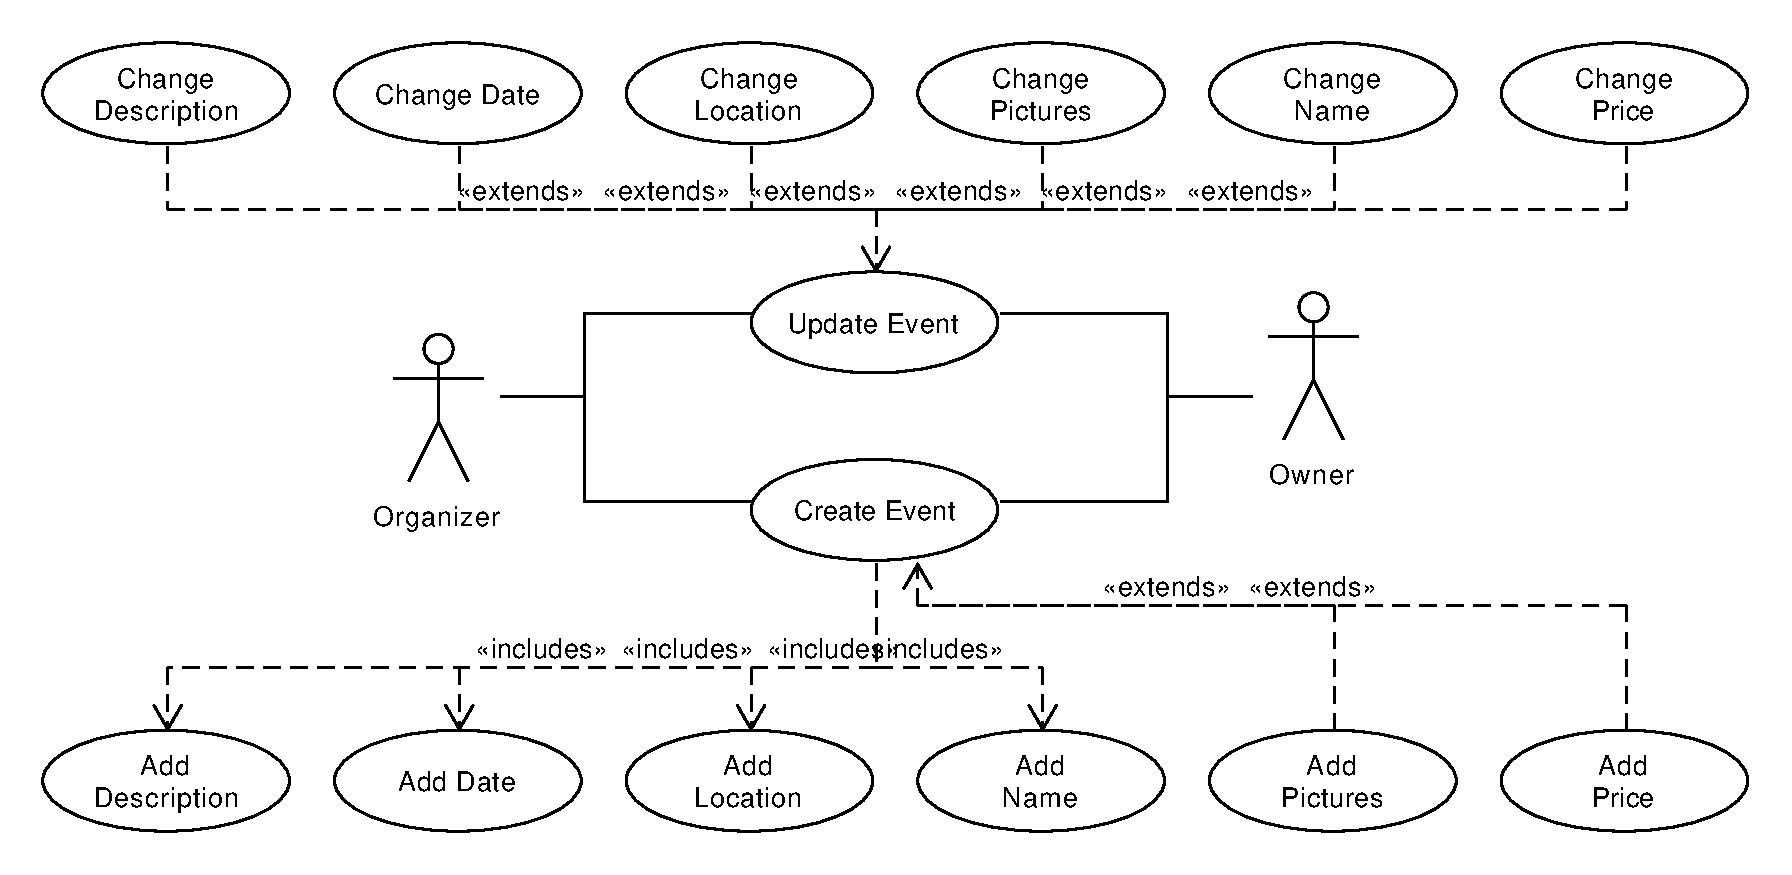
\includegraphics[width=\linewidth]{./images/FR8-10.pdf}
	\caption{UCD relativo a FR8 e FR10.}
	\label{fig:UCD_FR8-10}
\end{figure}

\subsubsection*{Use Case FR8: Creazione Eventi}

\textbf{Riassunto}

Lo use case in questione descrive come un utente appartenente alla categoria "Organizer" oppure "Owner" può creare nuovi eventi.

\newpage

\textbf{Descrizione}

\begin{itemize}
	\item Qualora l'utente appartenga alla categoria "Owner" o a quella "Organizer" e sia loggato (vedi \hyperref[Eccezioni-FR8-10]{Eccezioni}), dalla pagina del profilo personale è visibile un pulsante "New event"
	\item La pressione del pulsante rimanda alla pagina di creazione eventi. Per la creazione di un nuovo evento è necessario l'inserimento di un nome, di una data, di una location e di una descrizione (vedi \hyperref[Eccezioni-FR8-10]{Eccezioni})
	\item L'aggiunta di immagini è facoltativa, così come lo è il prezzo 
\end{itemize}

\subsubsection*{Use case FR10: Modifica Eventi}

\textbf{Riassunto}

Lo use case in questione descrive come un utente appartenente alla categoria "Organizer" oppure "Owner" può modificare eventi precedentemente creati.

\textbf{Descrizione}
\begin{itemize}
	\item Qualora un utente appartenente alle categorie "Owner" o "Organizer" sia loggato e abbia precedentemente creato un evento (vedi \hyperref[Eccezioni-FR8-10]{Eccezioni}), dalla propria pagina personale può raggiungere l'evento in questione tramite il pulsante "My events"
	\item La pressione del pulsante rimanda ad una lista degli eventi creati. Selezionandone uno è possibile modificare uno qualsiasi dei vari campi entro una settimana dall'evento (vedi \hyperref[Eccezioni-FR8-10]{Eccezioni} e \hyperref[Estensioni-FR8-10]{Estensioni})
\end{itemize}

\subsubsection*{Eccezioni}\label{Eccezioni-FR8-10}

\begin{itemize}
	\item Qualora l'utente non sia loggato, non esiste alcun profilo personale
	\item Qualora l'utente appartenga alla categoria "User", la pagina del profilo personale è priva del pulsante per la creazione di eventi
	\item Se durante la creazione di un evento non viene compilato uno dei campi obbligatori, il pulsante "Create Event" rimane inattivo
	\item Qualora l'utente non abbia mai creato eventi, il pulsante "My Events" non è attivo
	\item Qualora manchi meno di una settimana all'evento in questione, i campi non risultano modificabili
\end{itemize}

\subsubsection*{Estensioni}\label{Estensioni-FR8-10}

\begin{itemize}
	\item Gli eventi passati rimangono visualizzabili tramite il pulsante "My events", tuttavia non risultano più editabili
\end{itemize}


\subsection{FR12-13: Aggiunta e Modifica Luogo}


\begin{figure}[!htb]
	\centering
	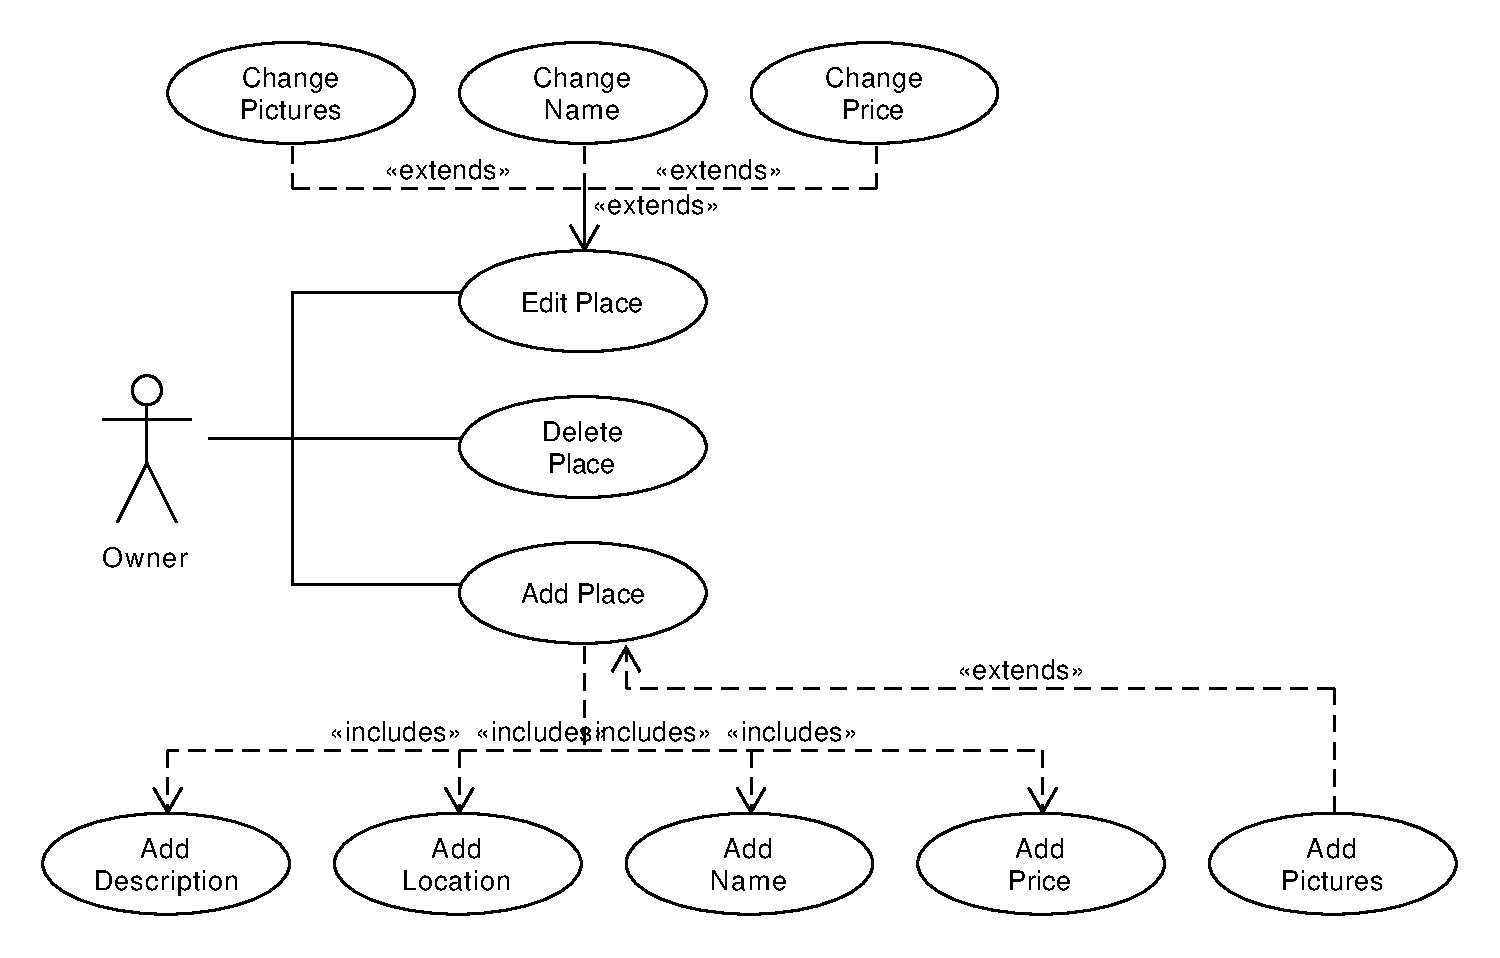
\includegraphics[width=\linewidth]{./images/FR12.pdf}
	\caption{UCD relativo al FR12.}
	\label{fig:UCD_FR12}
\end{figure}

\subsubsection*{Use Case FR12: Aggiunta Luogo}

\textbf{Riassunto}

Lo use case in questione descrive come un utente appartenente alla categoria "Owner" può aggiungere una location.

\textbf{Descrizione}

\begin{itemize}
	\item Qualora l'utente sia loggato con un profilo di tipo "Owner" (vedi \hyperref[Eccezioni-FR12-13]{Eccezioni}), dal proprio profilo personale ha la possibilità di aggiungere un luogo tramite il pulsante "New Place"
	\item La pressione del pulsante rimanda alla pagina di aggiunta luoghi. Per l'aggiunta di un nuovo luogo occorre inserire una location, un nome, una descrizione, ed un prezzo (vedi \hyperref[Eccezioni-FR12-13]{Eccezioni}). Opzionalmente è possibile inserire delle foto
\end{itemize}

\subsubsection*{Use Case FR13: Modifica Luogo}

\textbf{Riassunto}

Lo use case in questione descrive come un utente appartenente alla categoria "Owner" può modificare una location precedentemente inserita nel sistema.

\textbf{Descrizione}

\begin{itemize}
	\item Qualora l'utente sia loggato con un profilo di tipo "Owner" e abbia precedentemente aggiunto una location, dalla propria pagina personale può raggiungere l'evento in questione tramite il pulsante "My places"
	\item La pressione del pulsante rimanda ad una lista degli spazi aggiunti. Selezionandone uno è possibile modificare uno qualsiasi dei campi e/o eliminare lo spazio se e solo se lo spazio non è attualmente collegato ad un evento (vedi \hyperref[Eccezioni-FR12-13]{Eccezioni})
\end{itemize}

\subsubsection*{Eccezioni}\label{Eccezioni-FR12-13}
\begin{itemize}
	\item Qualora l'utente non sia loggato, non esiste alcun profilo personale
	\item Qualora l'utente non appartenga alla categoria "Owner", la pagina del profilo personale è priva del pulsante per l'aggiunta di spazi
	\item Se durante l'aggiunta di uno spazio non viene compilato uno dei campi obbligatori, il pulsante "Create Place" rimane inattivo
	\item Qualora lo spazio sia collegato ad un evento, le modifiche sono disattivate a partire da 7 giorni prima della data prevista per l'evento
\end{itemize}

\newpage
\section{Sequence and Activity Diagram}

Gli use case diagrams riportati nel capitolo precendente rappresentano una overview delle funzionalità del sistema. Nel presente capitolo tali funzionalità vengono estese tramite l'introduzione di un aspetto temporale. L'impiego di sequence diagrams consente quindi di rappresentare l'ordine cronologico con cui i vari elementi dei singoli scenari si verificano, dettagliando il modo in cui gli oggetti collaborano al fine di ottenere la piena funzionalità del sistema.

\textbf{Login}
\begin{figure}[!htb]
	\centering
	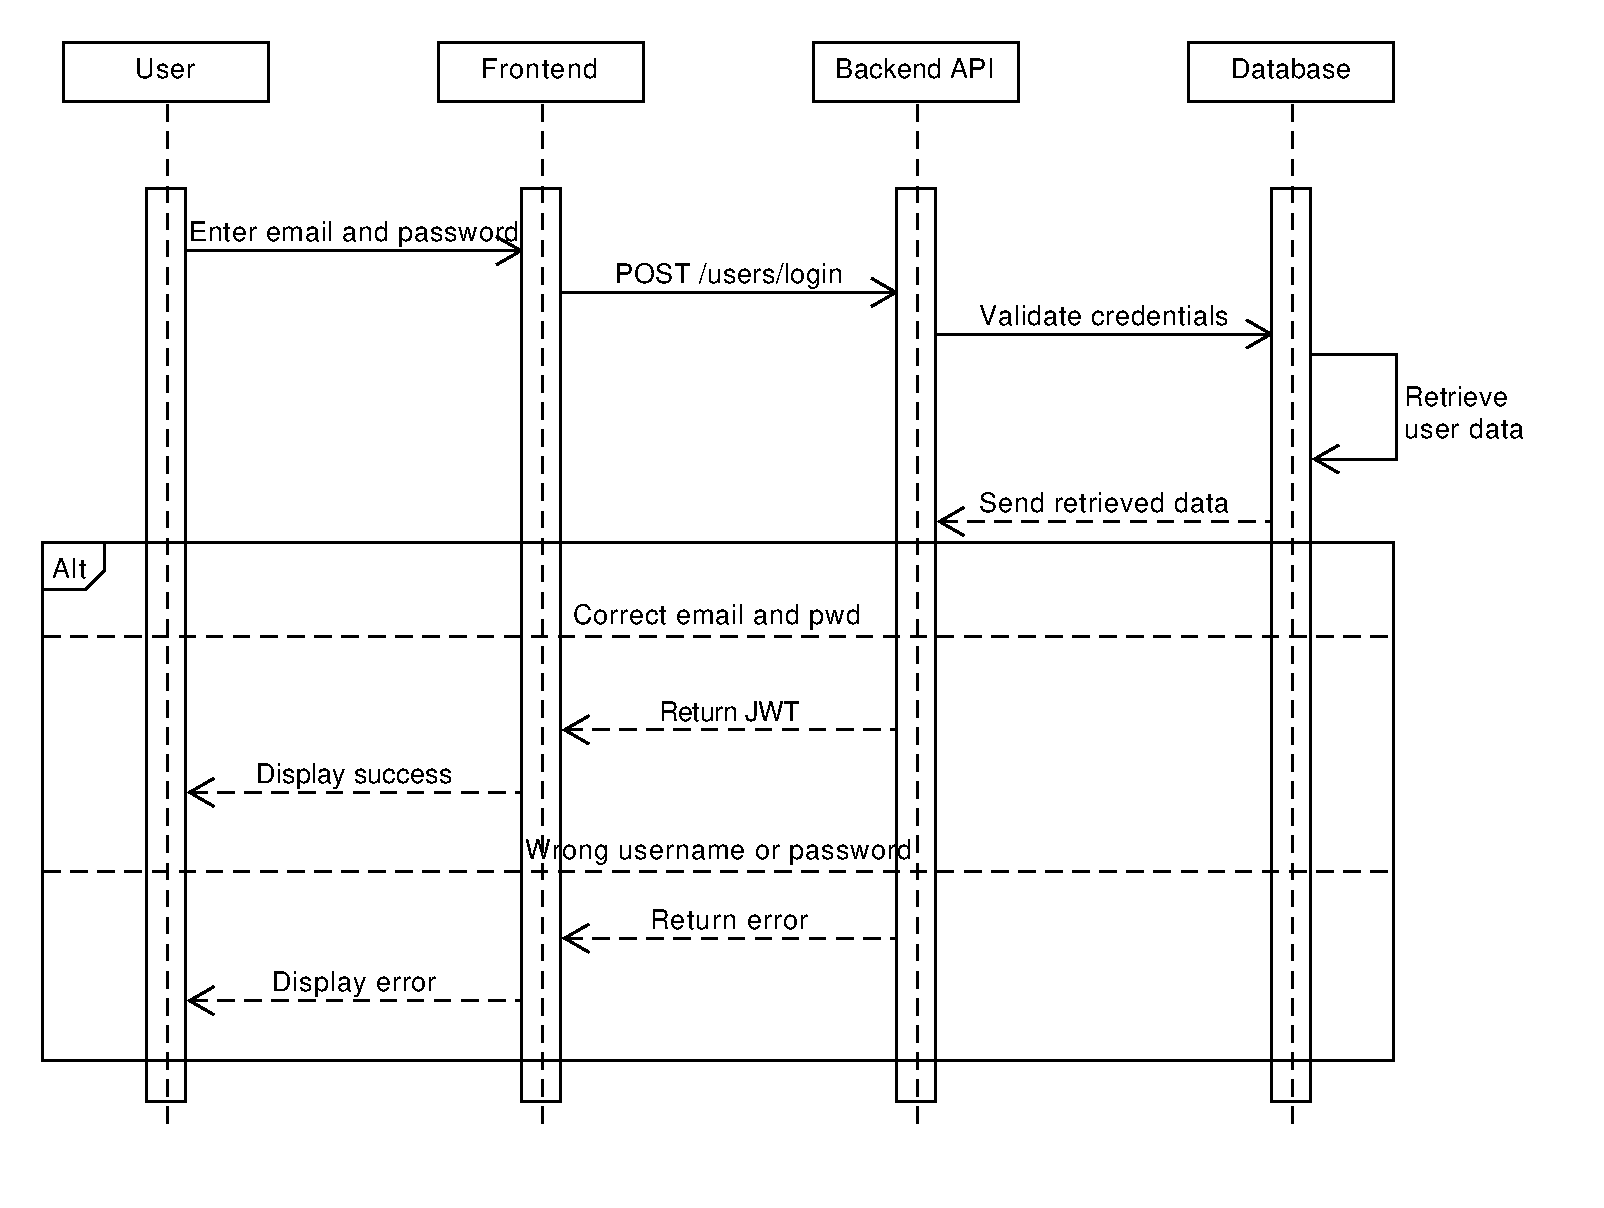
\includegraphics[width=\linewidth]{./images/SequenceDiagramLogin.pdf}
	\caption{Sequence diagram rappresentante la procedura di login.}
	\label{fig:SeqDiagLogin}
\end{figure}

\newpage
\textbf{Registrazione utente}
\begin{figure}[!htb]
	\centering
	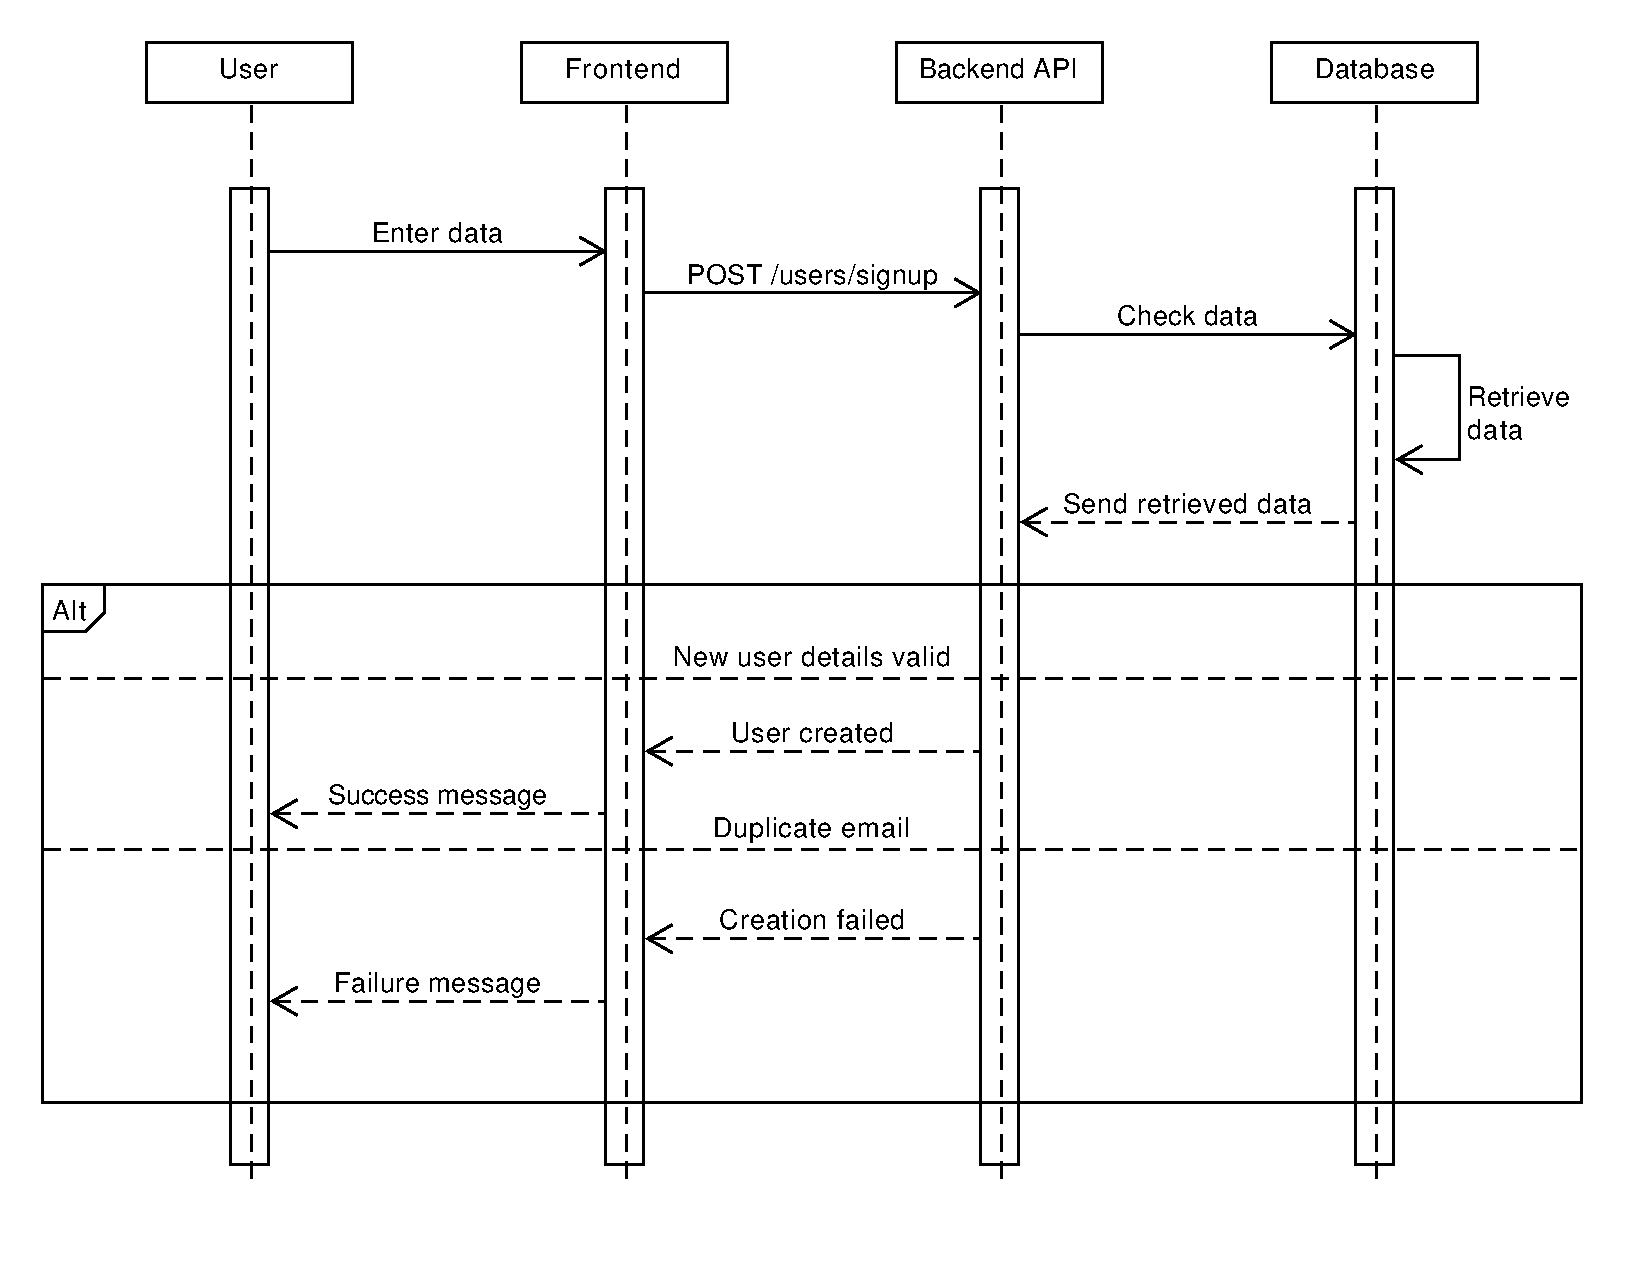
\includegraphics[width=\linewidth]{./images/SequenceDiagramRegistration.pdf}
	\caption{Sequence diagram rappresentante la procedura di registrazione.}
	\label{fig:SeqDiagReg}
\end{figure}

\newpage
\textbf{Browsing eventi}
\begin{figure}[!htb]
	\centering
	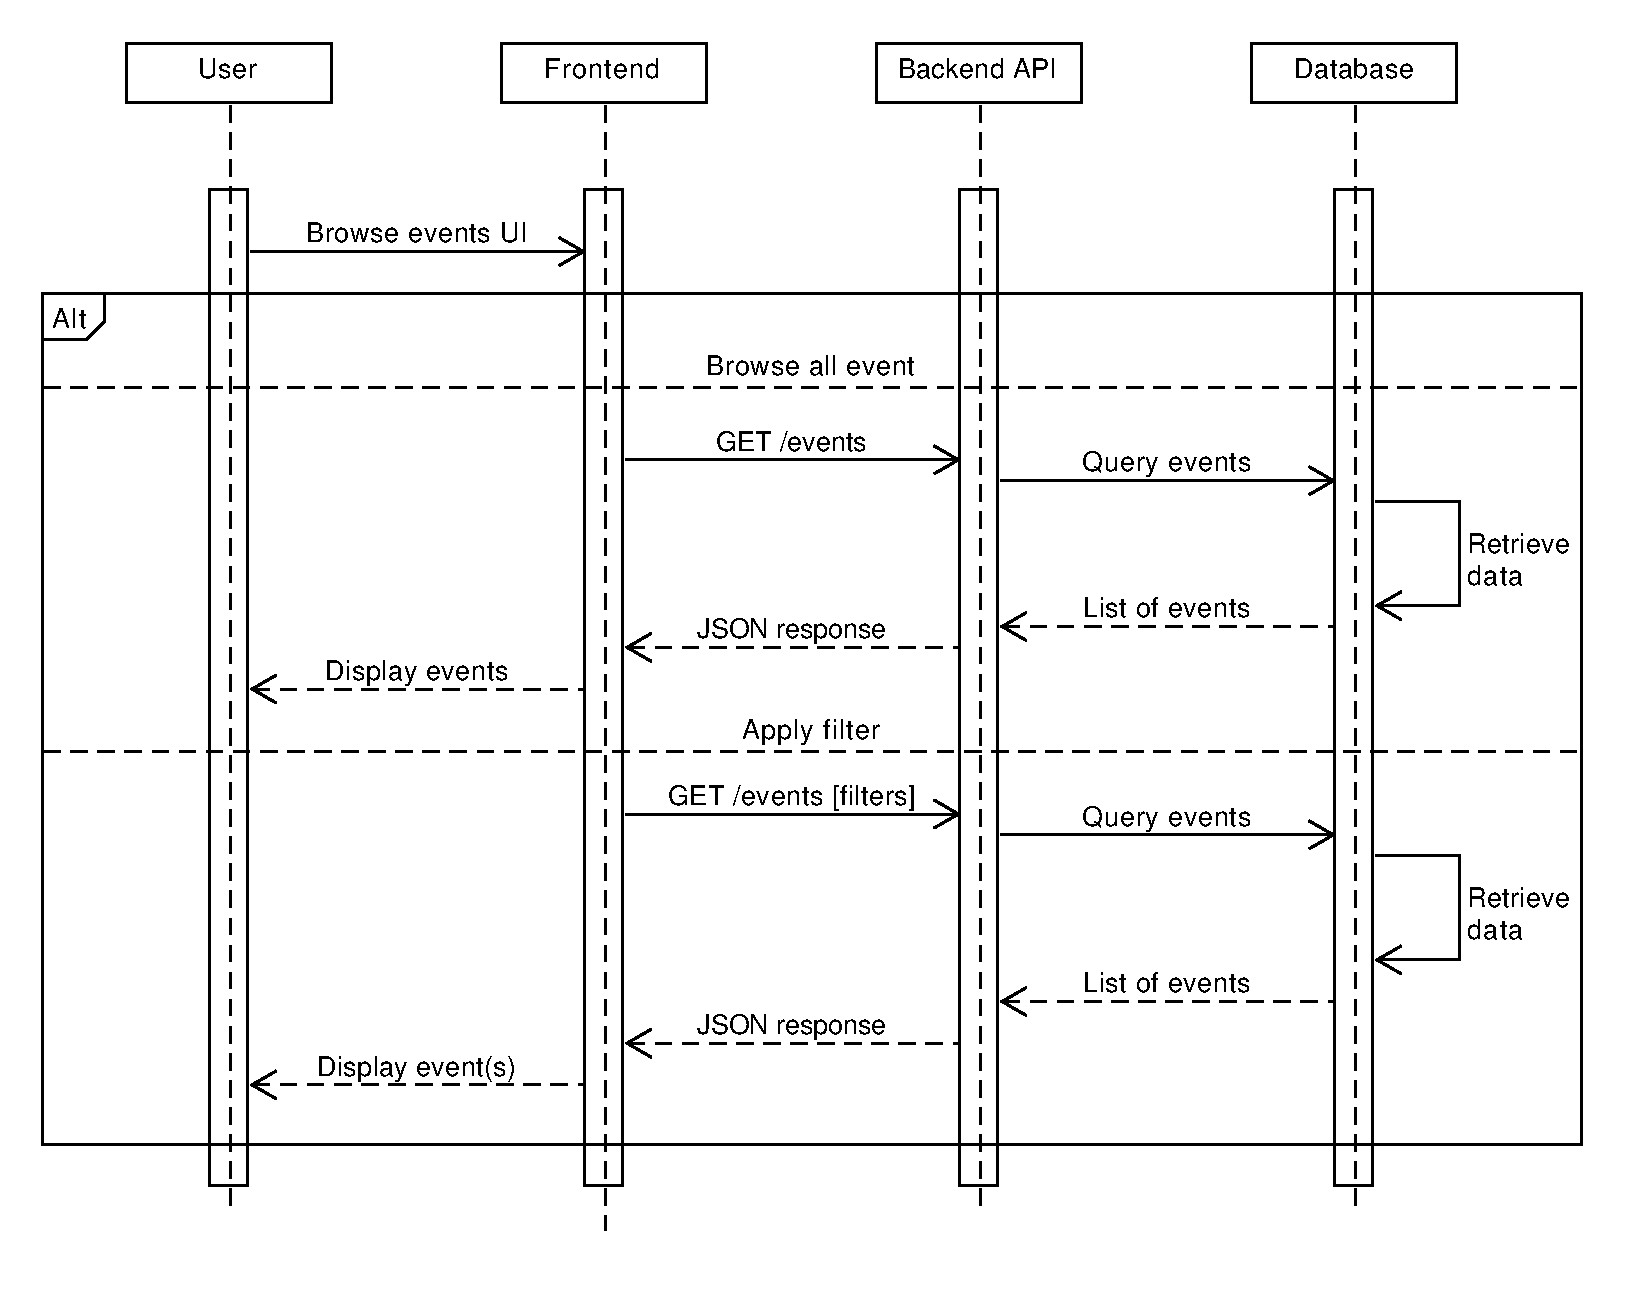
\includegraphics[width=\linewidth]{./images/SequenceDiagramBrowseEvents.pdf}
	\caption{Sequence diagram rappresentante il browsing degli eventi.}
	\label{fig:SeqDiagBrowseEvents}
\end{figure}

\newpage
\textbf{Iscrizione ad un evento}
\begin{figure}[!htb]
	\centering
	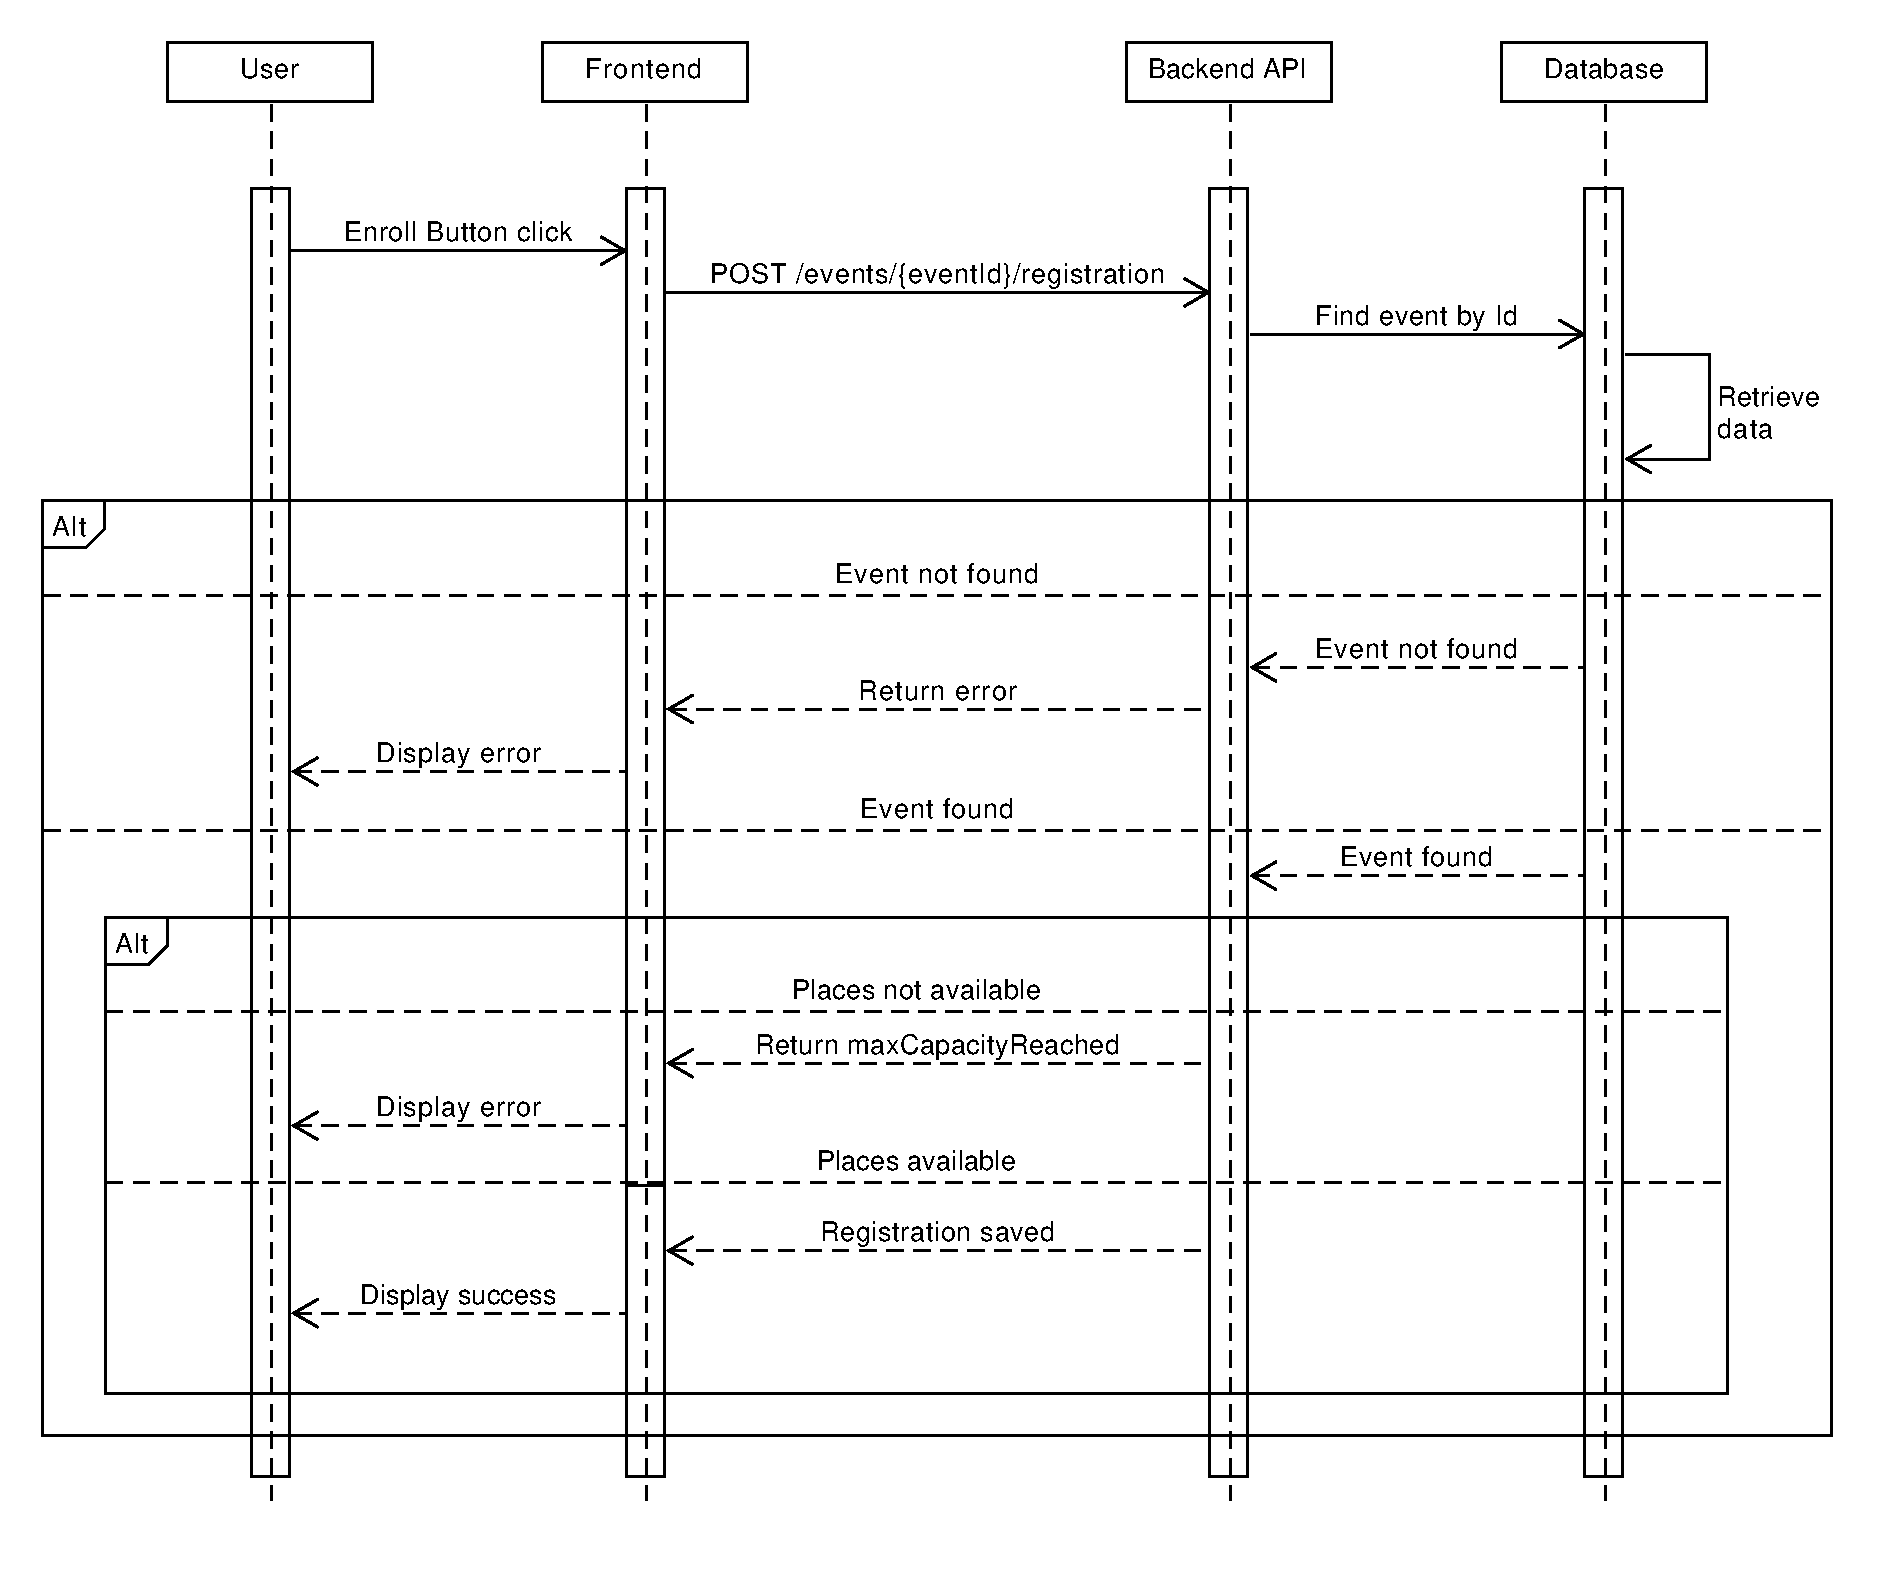
\includegraphics[width=\linewidth]{./images/SequenceDiagramEventEnrolling.pdf}
	\caption{Sequence diagram rappresentante l'iscrizione ad un evento.}
	\label{fig:SeqDiagEventEnroll}
\end{figure}

\newpage\textbf{Creazione di un evento}
\begin{figure}[!htb]
	\centering
	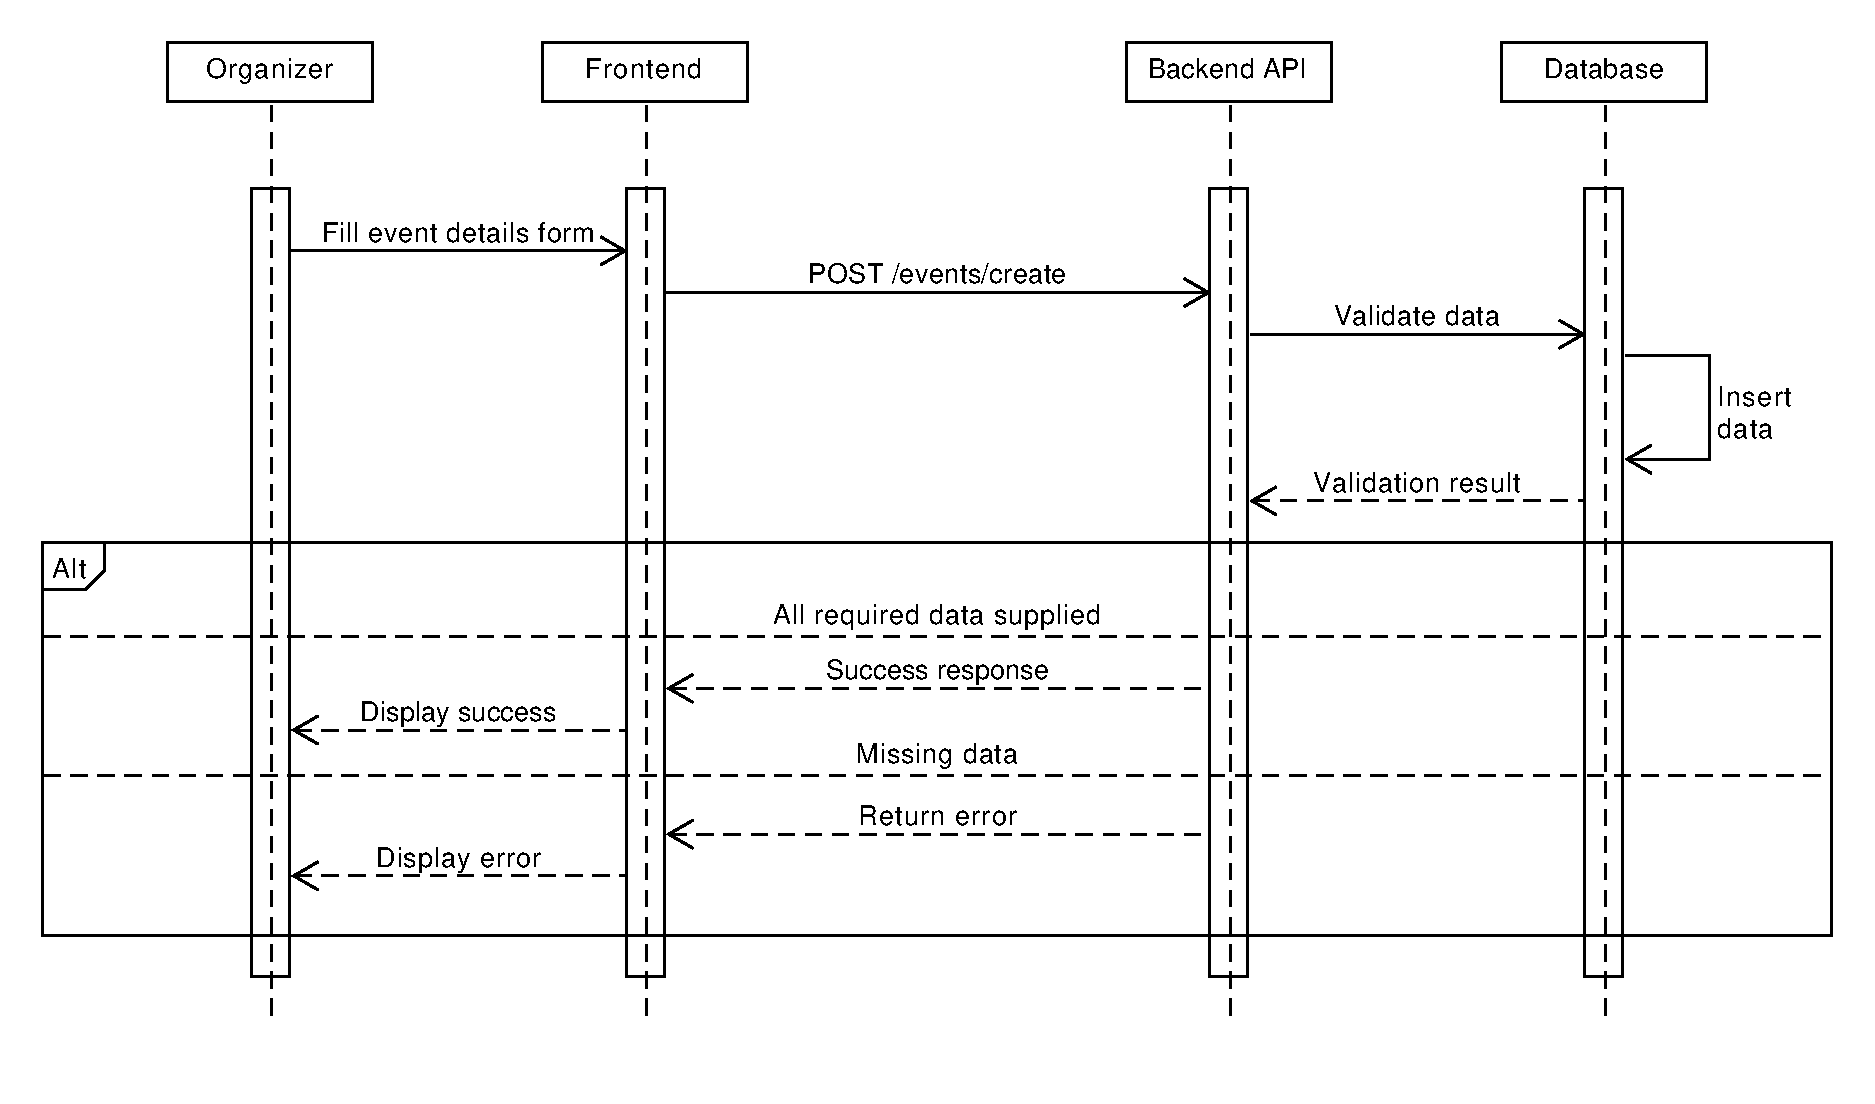
\includegraphics[width=\linewidth]{./images/SequenceDiagramEventCreation.pdf}
	\caption{Sequence diagram rappresentante la creazione di un evento.}
	\label{fig:SeqDiagEventCreation}
\end{figure}

\newpage
\textbf{Eliminazione di un evento}
\begin{figure}[!htb]
	\centering
	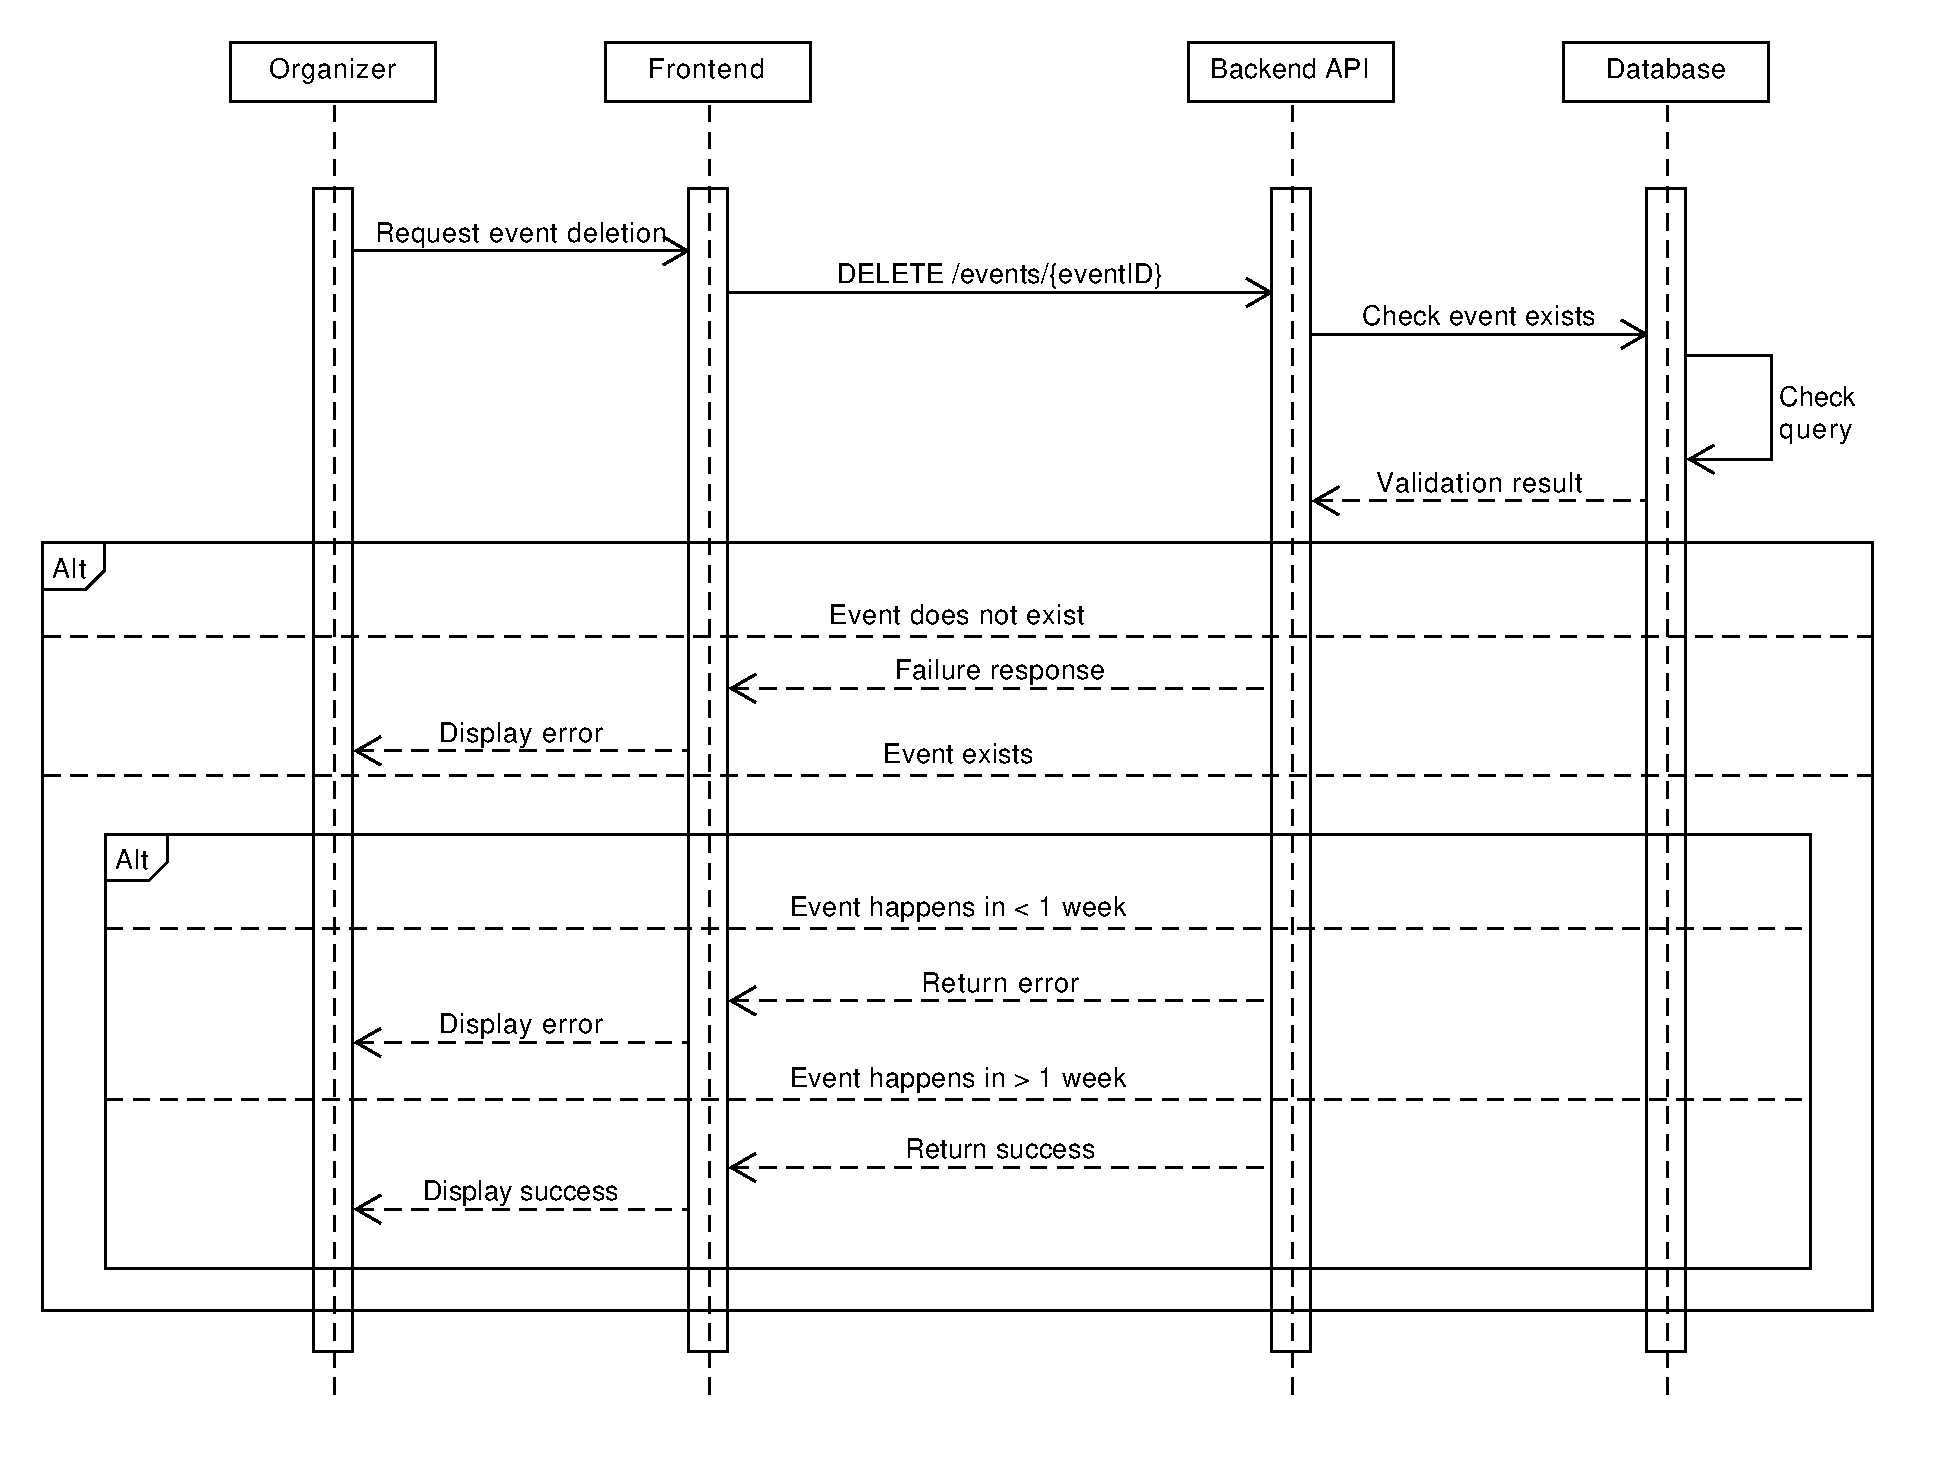
\includegraphics[width=\linewidth]{./images/SequenceDiagramEventDeletion.pdf}
	\caption{Sequence diagram rappresentante la reimozione di un evento creato in precedenza.}
	\label{fig:SeqDiagEventDeletion}
\end{figure}

\newpage
\textbf{Modifica di un evento}
\begin{figure}[!htb]
	\centering
	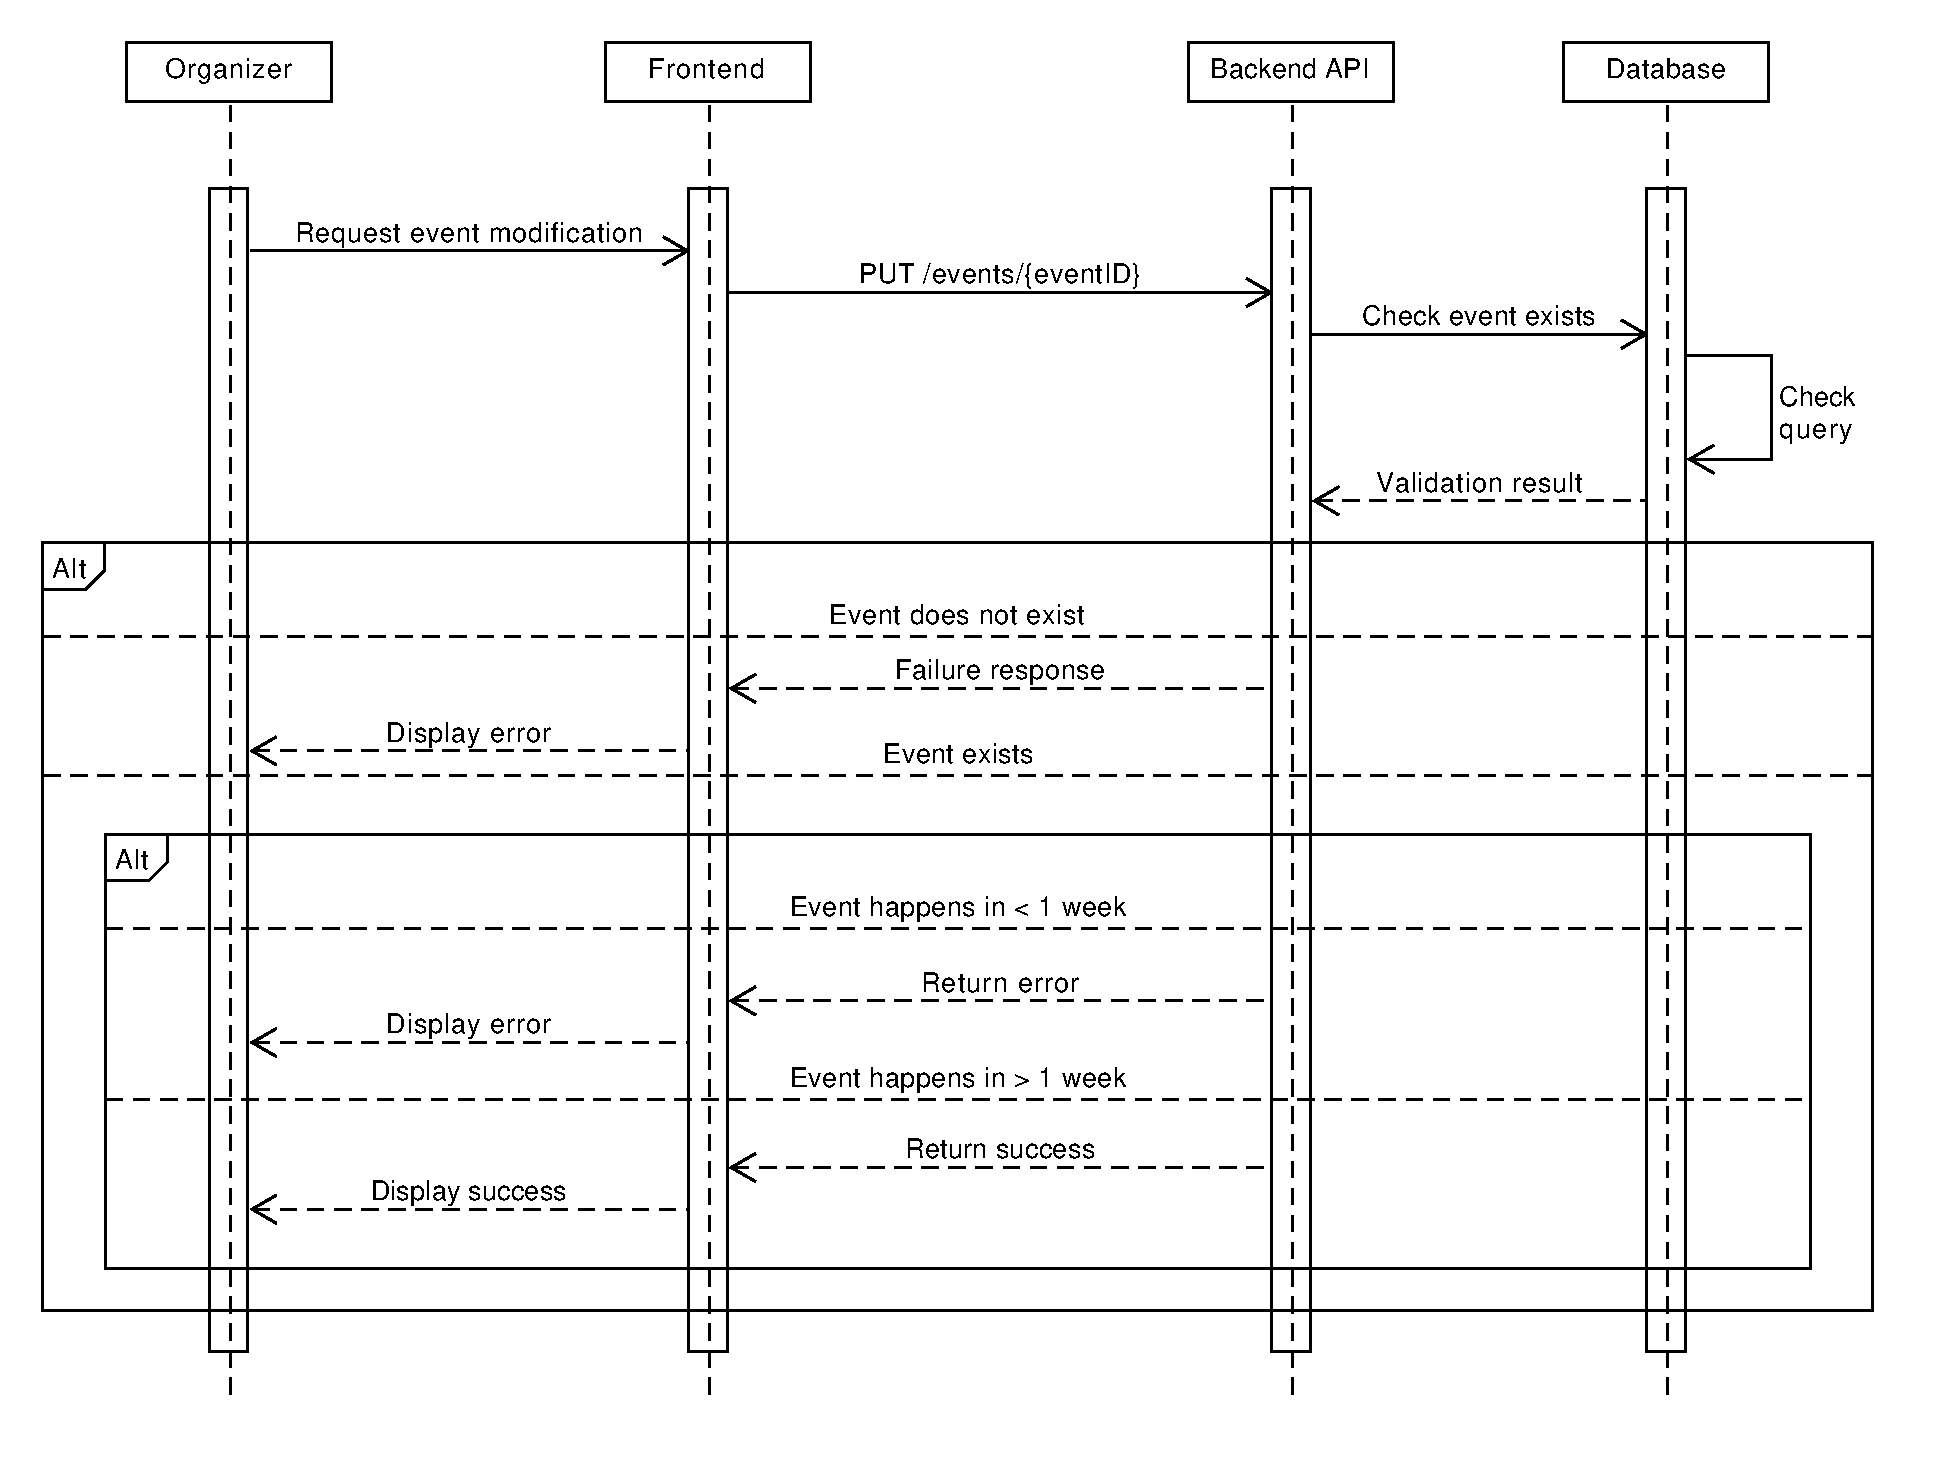
\includegraphics[width=\linewidth]{./images/SequenceDiagramEventModification.pdf}
	\caption{Sequence diagram rappresentante la modifica di un evento creato in precedenza.}
	\label{fig:SeqDiagEventModification}
\end{figure}

\newpage

\begin{itemize}
	\item add place
	\item remove place
	\item edit place
\end{itemize}

\newpage
\section{Analisi dei Componenti}

In questo capitolo vengono presentati i componenti che costituiscono l'architettura del sistema, e che sottostanno alle funzionalità definite in precedenza. L'interconnessione tra i vari componenti è rappresentata tramite l'utilizzo di un component diagram, il quale rende esplicita la presenza di interfacce sia tra i componenti  stessi che con sistemi esterni.


\subsection{Definizione dei Componenti}


\subsection{Diagramma dei Componenti}

\section{Diagramma delle Classi}




	
\end{document}